\section{Literature Review}

Other papers researching bus journey predictions look at a wide variety of models and factors affecting the journey time. This project focuses on bus journeys in London, however, it was not possible to find papers that also looked into modelling bus journeys in London. The results and findings presented below are all for regions outside London and therefore, care must be taken to apply the conclusions drawn from these papers directly to this project. Table \ref{table:lit-review-summary} shows a summary of the research papers that were studied. \\

Patnaik et al. developed a set of regression models to estimate the arrival times for buses travelling between two points. They used data collected by automatic passenger counters (APC) installed on buses in North-East United States of America \cite{apc-estimation}. For their model, they chose the following variables as independent variables: distance, number of stops, dwell times, number of boarding and alighting passengers and weather descriptors. They hypothesised that their results could have been improved if they had combined a Kalman Filter Model with their existing Regression Model. \\

Fan and Gurmu studied historical average models, Kalman Filter models and artificial neural networks (ANN) as the three models for predicting bus arrival times \cite{dynamic-gps}. It was discovered that the Kalman Filter model gave the better prediction in a lot of the time intervals. It was hypothesised that this was because the model always uses the current measurement to predict the next step. However, the model was found to be vulnerable where there were huge differences in travel times between two consecutive time periods, perhaps because it struggled to filter out noise as smoothly and so was not as capable of handling abrupt changes between consecutive travel times. Although the ANN model did not get the best predictions in most of the time intervals, overall it provided the best prediction in both accuracy and robustness. This is possibly because the ANN could handle the differences in travel times between time periods and so gave relatively stable prediction during both peak and off-peak hours. However, it was also found that the ANN model was less effective in predicting bus travel times for very short and/or very long trips. This could be because very short trips have high percentage errors. \\

Sun et al. used a Kalman Filter model to analyse their data for real-time bus arrival time predictions \cite{smart-public-transport}. They discovered that as the length of time from which the historical real time data is used (e.g. using the data collected from the past two hours as opposed to historical data from last week), increases from 30 minutes to 90 minutes, the model has a vast improvement on accuracy. However, the performance increase begins to plateau as the length of time increases any further, with the model's accuracy flat lining when the time window goes beyond 120 minutes. This indicates that only data within the last 120 minutes is significant for real time delay prediction. It was also discovered that the prediction performance of the models worsened as the prediction is applied further in the future. 

\begin{table}[H]
   \begin{tabular}{|l|l|l|l|l|}
\hline
\textbf{Author(s)}                                                               & \textbf{Location}                                                                                & \textbf{\begin{tabular}[c]{@{}l@{}}Model \\ Developed\end{tabular}}                                               & \textbf{\begin{tabular}[c]{@{}l@{}}Factors Affecting \\ Journey Times\end{tabular}}                                                                                                                           & \textbf{Findings}                                                                                                                                                                                      \\ \hline
\begin{tabular}[c]{@{}l@{}}Patnaik \\ et al.\end{tabular}                        & \begin{tabular}[c]{@{}l@{}}North \\ East,\\ USA\end{tabular}                                     & \cellcolor[HTML]{CBCEFB}\begin{tabular}[c]{@{}l@{}}Multivariate \\ Regression \\ Model\end{tabular}               & \cellcolor[HTML]{CBCEFB}\begin{tabular}[c]{@{}l@{}}distance travelled, \\ dwell times, number \\ of boarding and \\ alighting passengers, \\ weather descriptors, \\ day of week, time \\ of day\end{tabular} & \cellcolor[HTML]{CBCEFB}\begin{tabular}[c]{@{}l@{}}weather and day \\ of week are not \\ significant. time of \\ day, distance and dwell \\ times are significant.\end{tabular}                        \\ \hline
                                                                                 &                                                                                                  & \cellcolor[HTML]{C6DEFF}\begin{tabular}[c]{@{}l@{}}Historical \\ average \\ of all \\ collected data\end{tabular} & \cellcolor[HTML]{C6DEFF}\begin{tabular}[c]{@{}l@{}}time of day, correlation \\ of travel times of \\ successive journeys\end{tabular}                                                                         & \cellcolor[HTML]{C6DEFF}\begin{tabular}[c]{@{}l@{}}Outperformed by \\ ANN and Kalman \\ Model\end{tabular}                                                                                             \\ \cline{3-5} 
                                                                                 &                                                                                                  & \cellcolor[HTML]{FFFC9E}\begin{tabular}[c]{@{}l@{}}Kalman Filter \\ Model\end{tabular}                            & \cellcolor[HTML]{FFFC9E}time of day                                                                                                                                                                           & \cellcolor[HTML]{FFFC9E}\begin{tabular}[c]{@{}l@{}}Good prediction with\\ reasonable accuracy\end{tabular}                                                                                             \\ \cline{3-5} 
\multirow{-3}{*}{\begin{tabular}[c]{@{}l@{}}Fan and \\ Gurmu\end{tabular}}       & \multirow{-3}{*}{\begin{tabular}[c]{@{}l@{}}Macae, \\ Rio de \\ Janeiro, \\ Brazil\end{tabular}} & \cellcolor[HTML]{CDFFC9}\begin{tabular}[c]{@{}l@{}}Artificial \\ Neural\\ Network \\ (ANN)\end{tabular}           & \cellcolor[HTML]{CDFFC9}time of day                                                                                                                                                                           & \cellcolor[HTML]{CDFFC9}\begin{tabular}[c]{@{}l@{}}Relatively stable \\ prediction during peak \\ and off-peak hours. \\ Outperforms Kalman \\ model.\end{tabular}                                     \\ \hline
Sun et al.                                                                       & \begin{tabular}[c]{@{}l@{}}Nashville, \\ USA\end{tabular}                                        & \cellcolor[HTML]{FFFC9E}\begin{tabular}[c]{@{}l@{}}Kalman Filter \\ Model\end{tabular}                            & \cellcolor[HTML]{FFFC9E}\begin{tabular}[c]{@{}l@{}}time of day, \\ day of week\end{tabular}                                                                                                                   & \cellcolor[HTML]{FFFC9E}\begin{tabular}[c]{@{}l@{}}Looking at data in the past \\ 90 minutes gives good \\ results. Performance \\ worsens when data is from \\ more than 120 minutes ago\end{tabular} \\ \hline
                                                                                 &                                                                                                  & \cellcolor[HTML]{C6DEFF}\begin{tabular}[c]{@{}l@{}}Historical \\ average\end{tabular}                             & \cellcolor[HTML]{C6DEFF}\begin{tabular}[c]{@{}l@{}}traffic congestion, \\ dwell time at stops, \\ time of day, \\ day of week\end{tabular}                                                                    & \cellcolor[HTML]{C6DEFF}\begin{tabular}[c]{@{}l@{}}Outperforms regression\\ model.\end{tabular}                                                                                                        \\ \cline{3-5} 
                                                                                 &                                                                                                  & \cellcolor[HTML]{CBCEFB}\begin{tabular}[c]{@{}l@{}}Multivariate \\ Regression \\ Model\end{tabular}               & \cellcolor[HTML]{CBCEFB}\begin{tabular}[c]{@{}l@{}}traffic congestion, \\ dwell time at stops, \\ time of day, \\ day of week, \\ distance between \\ stops\end{tabular}                                      & \cellcolor[HTML]{CBCEFB}\begin{tabular}[c]{@{}l@{}}Hypothesised that there \\ might be nonlinear\\ relationships between the\\ arrival time and some of \\ the independent variables.\end{tabular}     \\ \cline{3-5} 
\multirow{-3}{*}{\begin{tabular}[c]{@{}l@{}}Jeong \\ and \\ Rilett\end{tabular}} & \multirow{-3}{*}{\begin{tabular}[c]{@{}l@{}}Texas, \\ USA\end{tabular}}                          & \cellcolor[HTML]{CDFFC9}\begin{tabular}[c]{@{}l@{}}Artificial \\ Neural\\ Network \\ (ANN)\end{tabular}           & \cellcolor[HTML]{CDFFC9}\begin{tabular}[c]{@{}l@{}}dwell time at stops, \\ time of day, \\ day of week\end{tabular}                                                                                           & \cellcolor[HTML]{CDFFC9}\begin{tabular}[c]{@{}l@{}}Outperforms historical and \\ regression model.\end{tabular}                                                                                        \\ \hline
\end{tabular}
    
    \caption{Summary of literature review findings}
    \label{table:lit-review-summary}
\end{table}

Jeong and Rilett studied historical average models, multivariate regression models and ANNs. This study found that the ANN model outperformed the other two models \cite{ann-prediction}. It was hypothesized that this was because the ANN was able to identify the complex nonlinear relationship between bus travel time and the independent variables. Jeong and Rilett also found that the historical model provided best predictions for `peak' hours. Their hypothesis behind this was that congestion made travel times consistently high, i.e. less variable.

\subsection{Factors Affecting Bus Arrival Times}
\label{factors-affecting-arrival-times}

There are a variety of different factors that can affect the arrival time of a bus, be that through affecting the travel time of the bus or the dwell time of the bus. In this case, the dwell time refers to time that a bus spends at a bus stop before it continues on its route. For example, the bus' travel time could be affected by traffic conditions. Similarly, the bus' dwell time could be affected if there are a large number of people that get on at the previous stop. Due to the sheer number of factors that could be investigated, this section will take a brief look at a selection of the factors that have been considered in other papers as well as some other factors that have the potential to be important. This section will provide justification for why some of the factors listed below do not warrant further investigation and do not need to be included in the models that will be developed. \\

It should be noted that most of the factors mentioned below are largely dependent upon one another. For example, the time of day could affect the traffic conditions (say rush hour leading to more vehicles on the road) or the weather could affect the dwell time (if it is particularly cold or icy, there may be fewer people willing to walk or cycle, so there are more people using buses). Therefore, care will have to be taken when implementing the models, to ensure that not too much weighting is placed on any singular factor. \\

The majority of research into bus journey predictions make use of data on traffic stream variables, for example weather, speed, distance \cite{dynamic-gps}. However, in the absence of such information and with limited resources, it is important to see if predictions made without this data can be made. Furthermore, it would be interesting to see if these predictions are comparable to those made with traffic stream information.

\subsubsection{Weather}

Koetse and Reitveld found that there is a substantial reduction in traffic speed when weather conditions are extreme \cite{weather-transport-effect}. In the presence of rain there was a decrease of up to 6\% in traffic speed, up to 13\% for snow and up to 12\% for reduced visibility. Slower traffic speeds means that vehicles will take longer to arrive at their destinations than usual and therefore, it can be argued that weather should be taken into account when creating models that predict bus arrival times. Furthermore, when temperatures are at the extremes, there is a case for people being more likely to take a bus than walking or cycling. Not only would this increase the load on the bus, leading to a slower bus speed, but the dwell time at the bus stops would also increase as more time would have to be taken for people to get on and off the buses. \\

It was found by Patnaik et al. that there was little to no effect between weather and bus delay time \cite{apc-estimation}. This finding was attributed to the fact that the weather data used in this investigation was not sufficiently detailed, or that during the study period the weather variations were not significant enough to have an impact on arrival times. 

\subsubsection{Time of Day and Time of Week}

It is hypothesised that at different times of day and different days of the week, there are different travel patterns. For example, at weekday rush hour times, there are more likely to be more vehicles on the road and thus more congestion. On the other hand, on weekends, there is less likely to be a strong correlation between time of day and late buses as there is not a particular time when a large proportion of the population has to travel somewhere. \\

Fan and Gurmu clustered their travel time data by time period and explored the effects of this. The results can be seen in Figure \ref{fig:time-of-day-week}, which plots the travel time index against the time of day \cite{dynamic-gps}. Here, the travel time index is the ratio of the average travel time per weekday and the average travel time across all days. An observation that was made was that in the evening rush hour (5 - 6 pm), the travel times were 30\% higher than the average across all time periods and days. This supports the idea of further exploring time of day as a parameter in the predicting of bus arrival times. \\

Fan and Gurmu also observed that the travel time distributions over the different days of the week seemed to be nearly the same. Therefore, since Figure \ref{fig:time-of-day-week} only shows data for weekdays, it could be argued that for weekdays, it will suffice to look at the effect of the time of day, without taking into account which day of the week it is. A similar concession can be made for weekends, i.e. the prediction model for Saturday 3pm should be no different to the prediction model for Sunday 3pm. However, Fan and Gurmu's findings are based on a model for a city in Brazil. It is unclear how strongly these findings would generalise to London. For example, the daily travel landscape in terms of when people leave work etc. may not be the same, or this city may not have bus lanes as in London.

\begin{figure}[H]
\begin{center}
    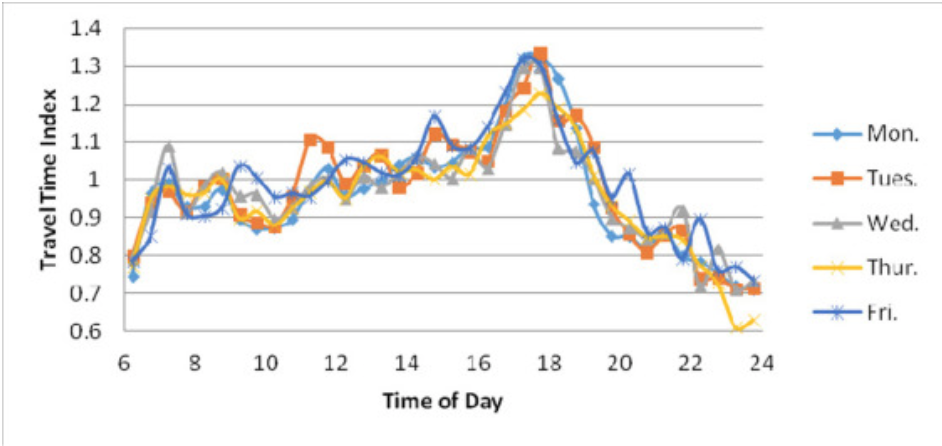
\includegraphics[keepaspectratio, width=12cm]{Images/day-time-of-week-effect.png}
    \caption{Effect of time of day and day of week, original image from \cite{dynamic-gps}}
    \label{fig:time-of-day-week}
\end{center}
\end{figure}

\subsubsection{Time of Year}

Similarly to the previous parameter, it is hypothesised that at different times of year, there are different travel patterns for buses. This could be due to factors such as special occasion (e.g. New Year's Day or bank holidays) or school holidays. For example, during term time, buses are not likely to have have the same travel time as during school holidays. \\

Since this project only runs from March to June, it was initially believed that there would not be a significant enough event that would lead to a marked change in bus travel times. However, due to the situation with COVID-19, London was placed officially in lockdown from March 24th 2020 and the public was heavily discouraged from using public transport. From March 16th 2020 people had been told to avoid all non essential contact with others and people were asked to work from home where possible \cite{london-lockdown-dates}. This dramatically reduced the load on the London transport network with the number of people using buses dropping by 85\% in April and May 2020 \cite{tfl-press-release-april}. Therefore, it was hypothesised that due to the lower number of vehicles on the road as well as the fewer number of people using buses, journey times would be shorter. As of May 18th 2020, TfL has begun to increase its bus services again, with the network running at 85\% capacity from this date \cite{tfl-press-release-may}. Furthermore, the government's new legislation means that from the 31st of May 2020, many of the previous restrictions are now being lifted. Therefore if data collected between March 24th 2020 and May 31st 2020 is labelled as lockdown data and data collected outside of these dates is labelled as pre/post lockdown data, then there should be enough data to adequately model this. \\

\subsubsection{Dwell Time at Bus Stops}

The amount of time a bus spends at a bus stop before continuing on its journey, also known as its dwell time, is one of the factors that have been considered to affect the arrival time of a bus. The dwell time of a bus can be affected by varying numbers of passengers at bus stops. For example, if a bus stop is outside a particularly popular destination, then the number of passengers getting off the bus would be higher than normal and thus the bus would have to wait at that particular stop for a longer amount of time. \\

Fan and Gurmu found that bus stop dwell times were less important and statistically not as significant as other potential factors affecting bus journey times \cite{dynamic-gps}. Furthermore, with the tools currently available, there is no real way to calculate how long a bus waits a single stop for. TfL does not currently provide any APIs that would directly give a bus' dwell time nor does it provide APIs that could aid in the calculation of dwell time, e.g. the number of passengers boarding or deboarding a bus. 

\subsubsection{Traffic Conditions}

Jeong and Rilett argued that in order to accurately predict bus travel time, it it essential to consider traffic conditions \cite{ann-prediction}. In June 2019 Google Maps introduced a new feature for forecasting bus delays by taking into account real time car traffic data and combining this with data on bus routes and stops \cite{google-machine-learning}. Both of these support the idea that traffic conditions should be considered as one of the parameters that affect bus arrival times. \\

However, Williams and Hoel found that daily traffic condition patterns were consistent across the weeks \cite{consistent-traffic}. This implies that if bus delays are affected by traffic, then historical bus travel times should not vary across the same time periods for different weeks. Therefore, traffic conditions do not need to be taken into account as a factor, especially for historical average models. \\

It can also be argued that the presence of bus only lanes means that there is little point in taking general traffic into account because traffic conditions will have less of an effect on the travel time of buses. However, bus lanes in London are occasionally occupied by other vehicles or road works, resulting in less smooth traffic in bus only lanes.

\subsection{Conclusions}

Following in Patnaik et al.'s example \cite{apc-estimation}, the effect of weather on bus arrival times will not be explored further. All the data that is used in this project has been collected manually since TfL does not provide any historical data on bus arrival times. Therefore, the collected data spans from mid March to early June. This is unlikely to be a large enough sample of different and extreme weather conditions to accurately identify and quantify the effects of differences in weather conditions. So, based off of Patnaik et al's findings, this supports the idea that weather would not be very suitable to be studied as a factor affecting bus arrival times in this particular project. \\

Time of day and day of week will be studied further as factors affecting bus journey times. Time of year generally is unlikely to be explored any further as a factor affecting bus arrival times because it is impossible to get a whole year's worth of data to use for modelling. However, the effect of COVID-19 lockdown on bus journey times will be considered further. \\

Since there is no way to get information on bus dwell times within the scope of this project, this factor will not be explored any further. However, this could be a possible extension or further work. Traffic conditions will also not be explored any further. \\

\clearpage